% !TeX root = RDT.tex
\documentclass[a4paper, 11pt]{article}    

\usepackage[ngerman]{babel}                   
\usepackage[onehalfspacing]{setspace}
\usepackage[top=2.5cm,bottom=2.5cm,left=2cm,right=2cm,marginparwidth=1.75cm]{geometry}

% Load useful packages                        
\usepackage{amsmath}                            
\usepackage{xcolor}                             
\definecolor{custom-blue}{RGB}{0,99,166} 
\usepackage{hyperref}
\hypersetup{colorlinks=true, allcolors=custom-blue}
\usepackage[default]{sourcesanspro}             
\usepackage[T1]{fontenc}                        
\usepackage{wrapfig}
\usepackage{fancyhdr}
\usepackage{longtable}
\usepackage{lastpage}
\usepackage{float}
\usepackage{tabularx} 
\usepackage[normalem]{ulem}
\useunder{\uline}{\ul}{}
\usepackage{booktabs}
\usepackage{graphicx}
\usepackage{color}
\usepackage{tabularray}
\usepackage{enumitem}
\usepackage{subcaption}


\pagestyle{myheadings}
\pagestyle{fancy}     

\definecolor{Alto}{rgb}{0.878,0.878,0.878}
\definecolor{Nobel}{rgb}{0.701,0.701,0.701}

\setlength{\headheight}{30pt}
\renewcommand{\headrulewidth}{0.5pt}
\renewcommand{\footrulewidth}{0.5pt}

\fancyhead[C]{}                                 
\fancyhead[R]{}                      
\fancyfoot[L]{}
\fancyfoot[C]{}                 
\fancyfoot[R]{\thepage/\pageref{LastPage}}

\title{
    MHS3D
}

\begin{document}

\maketitle
\clearpage

\tableofcontents
\clearpage

%
\section{Requirements}
\begin{enumerate}
    \item Die Smartwatch soll den MPU6050 Beschleunigungssensor + Gyroskop ansteuern und deren Messdaten abfragen können.
    \item Die von der Uhr gesammelten Messdaten sollen im laufenden Betrieb an einen PC übertragen werden können.
    \item Bewegungsrichtungen sollen live in 3D (als Linie im “Raum”) angezeigt werden.
    \item Das Bewegungstracking der letzten 2 Stunden soll während des Betriebs gespeichert und dargestellt werden können.

\end{enumerate}

Erweiterungsideen:
\begin{itemize}
    \item Der Puls des Trägers  wird als Liniendiagramm, gefärbt nach Bereichen, altersabhängig (grün bis rot) angezeigt werden.
    \item Pulsänderungen sollen als farbliche Veränderung des Bewegungsstriches im Raum visualisiert werden.
    \item Aufnahme der Daten in Sessions mit Button an der Uhr als Start/Stop
    \item Interaktive Drehung der Ansicht möglich
    \item Mapping der Bewegungen in die Raumpläne der HAW
\end{itemize}
\clearpage


\section{Projektplan}
\subsection{Projektaufbau}
Ein Projektplan der bei Konkretisierung und Arbeitsteilung nach dem Aufstellen der Anforderungen entstanden ist.

\begin{figure}[H]
    \centering
    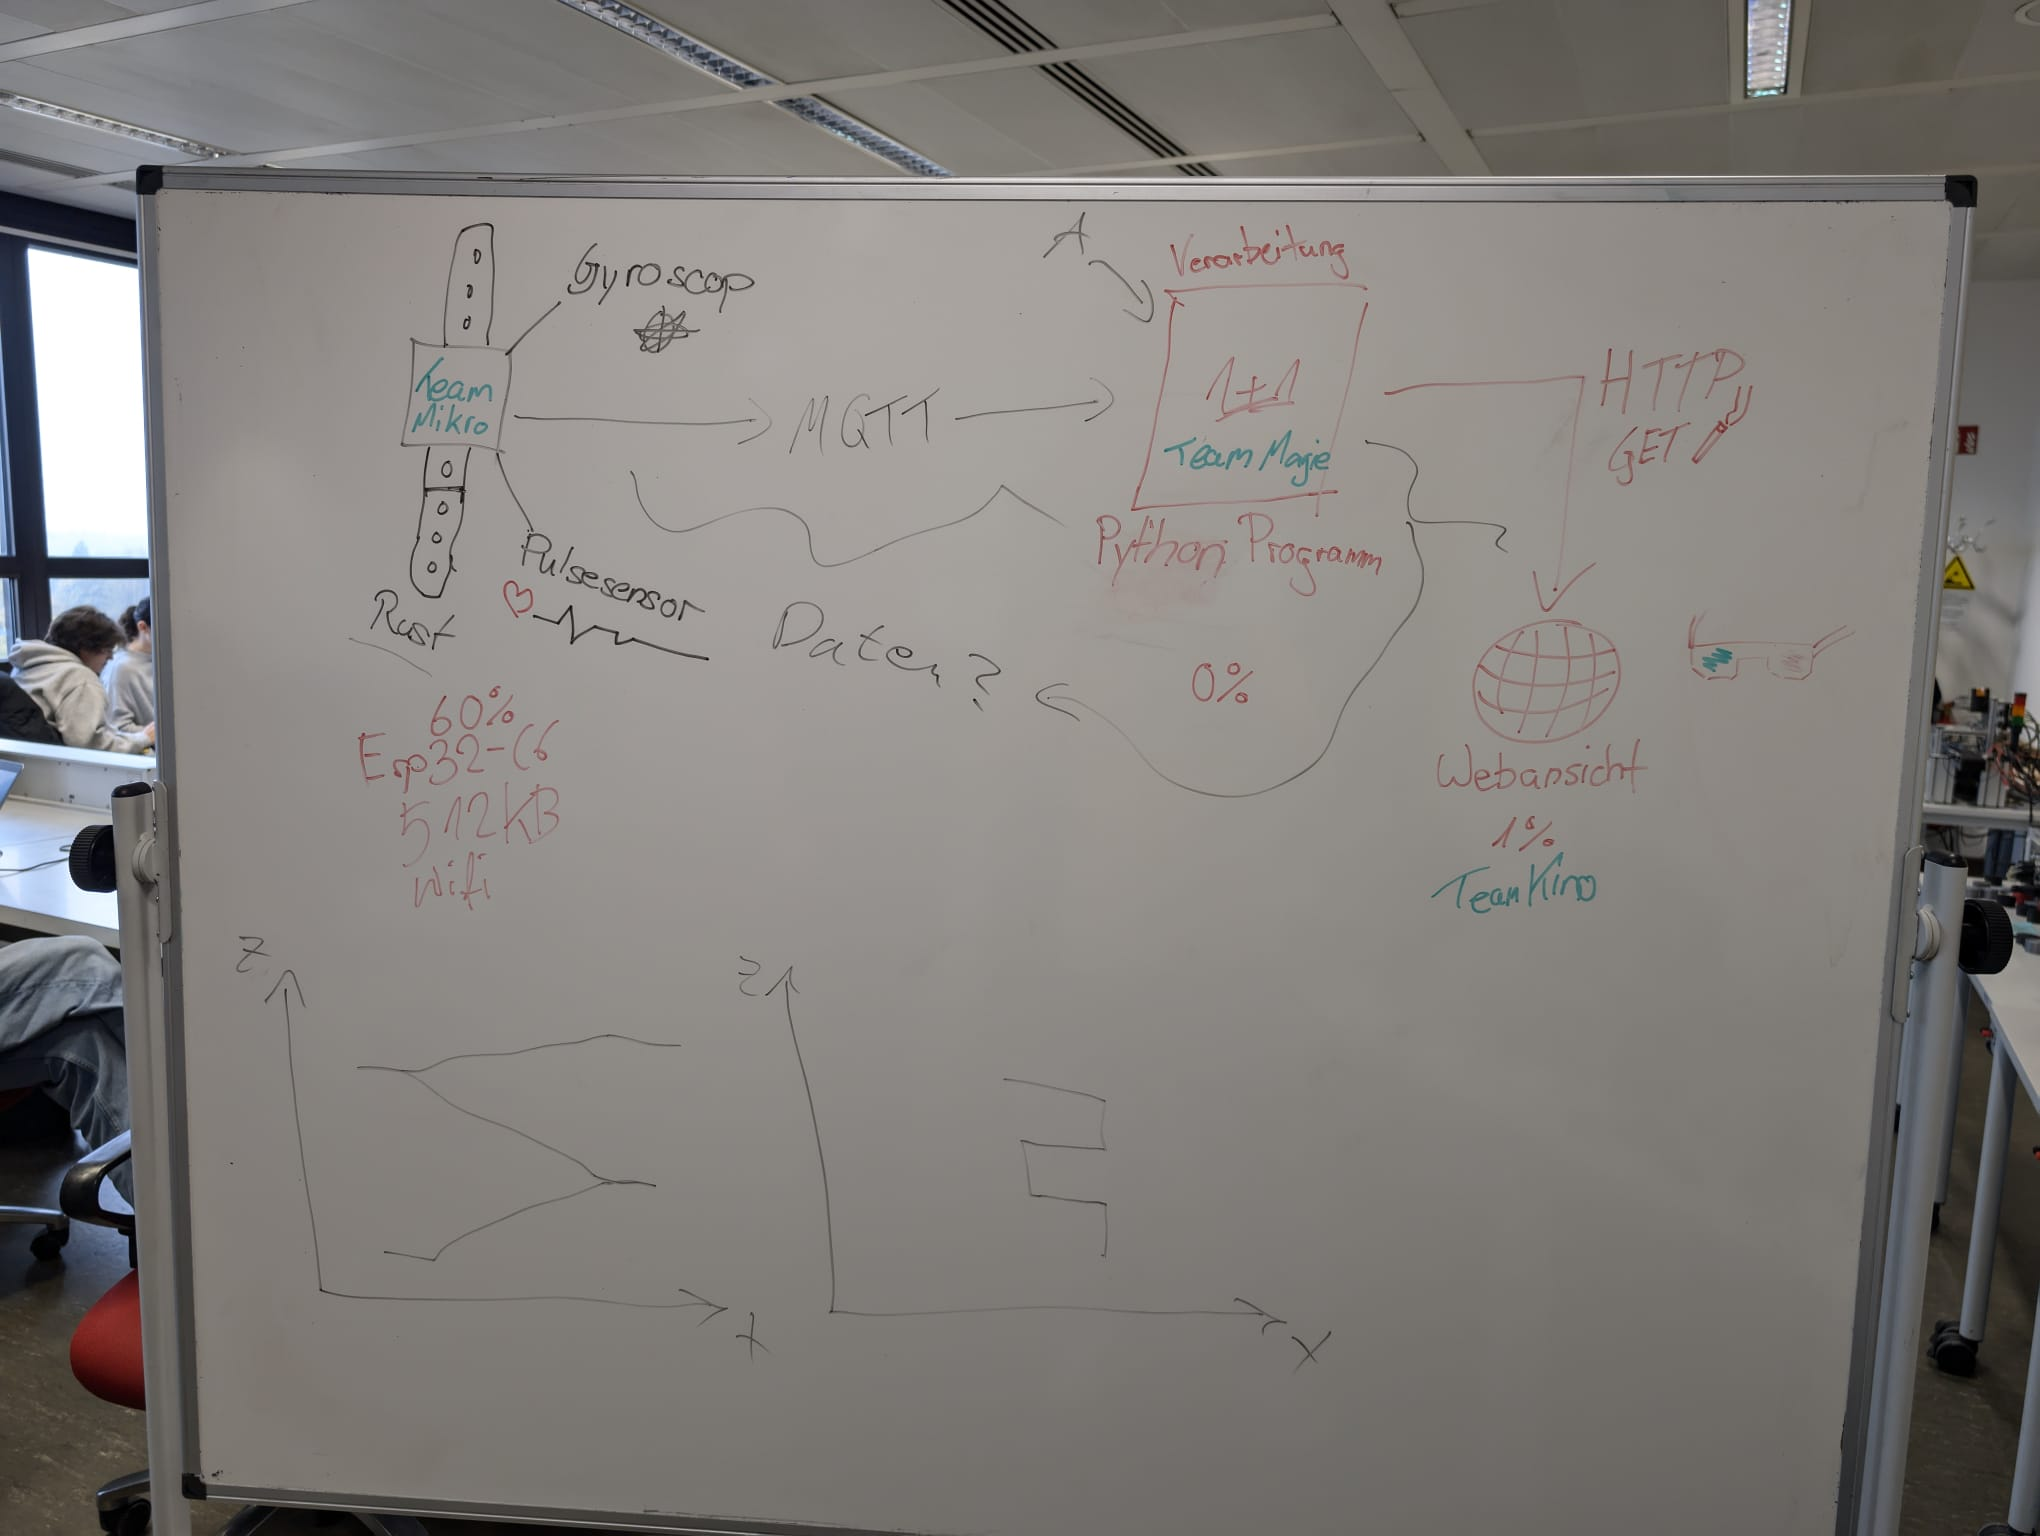
\includegraphics[width=0.7\textwidth]{images/Projektaufbau.jpeg}
    \caption{Projektaufbau}
    \label{fig:Projektaufbau}
\end{figure}
\noindent Die Idee war es mit der Uhr über die Sensorik Daten zu sammeln, diese per MQTT einem PC/Laptop zur Verfügung zu stellen und dort die gesammelten Daten aufzubereiten um diese dann in einer Webansicht darstellen zu können.

\noindent Nach der Gruppeneinteilung haben wir uns entschieden den Code für die Uhr in Rust zu schreiben, die Datenaufbereitung in Python zu machen und diese Daten per HTTP einem Javaprogramm zur Darstellung zugänglich zu machen.

\noindent (vermutlich um angepassten digitalen Projektaufbau ergänzen/ersetzen und Änderungsgründe erläutern)


\clearpage
\subsection{grober Zeitplan}
Ein grober Zeitplan der Recherche und Umsetzung des Projektplans den wir zu Anfang der Planung geschrieben haben.
\begin{center}
    \begin{tabularx}{\textwidth}{ |c|X|X|X| }
        \hline
        \textbf{KW} & \textbf{Micro}                                    & \textbf{Magic}        & \textbf{Kino}                            \\
        \hline
        \textbf{44} & Projekt aufsetzen                                 &                       &                                          \\
        \hline
        45          & Sendemethode festlegen                            & Recherche Algorithmen & Recherche: Darstellung Was und Wie?      \\
        \hline
        \textbf{46} & Format der Daten festlegen                        &                       & Mockups erstellen                        \\
        \hline
        47          &  Gyroskopdaten aufnehmen                          &                       & Aufsetzen des Frontends                  \\
        \hline
        \textbf{48} & Accelerationdaten aufnehmen                       &                       &                                          \\
        \hline
        49          & Stetige Anpassung an Bedürfnisse                  &                       & Testen der Darstellung mit Dummy-Daten   \\
        \hline
        \textbf{50} &                                                   &                       &                                          \\
        \hline
        51          &                                                   &                       & Daten von Magic empfangen und darstellen \\
        \hline
        \textbf{54} &                                                   &                       &                                          \\
        \hline
        55          &                                                   &                       & Testen                                   \\
        \hline
        \textbf{56} &                                                   &                       &                                          \\
        \hline
        57          &                                                   &                       &                                          \\
        \hline
    \end{tabularx}
\end{center}

\subsection{Erfahrungen von Team Micro}

\subsubsection{Beschreibung des Vorgehens:}

\begin{enumerate}
    \item Die Uhr wurde mit einem ESP32C6 Mikrocontroller aufgebaut, der die Sensoren ansteuert und die Daten sammelt.
    \item Die Daten werden in einem JSON Format an den PC gesendet.
    \item In der Entwicklung nutzen wir die Programmiersprache Rust. Dies hatte mehrere Gründe:
    \begin{enumerate}
        \item Rust ist eine Systemsprache, die eine hohe Geschwindigkeit und Sicherheit bietet.
        \item Rust ist eine moderne Sprache, die viele Features bietet, die die Entwicklung erleichtern.
        \item Sowohl Laurin, als auch Tom haben in den letzten Semestern sehr viel mit Rust gemacht und sind daher vertraut mit der Sprache.
        \item Eine interessante Herausforderung, da Rust verglichen mit C noch nicht so weit verbreitet ist bei der Mikrocontrollerprogrammierung.
        \item Weils Spaß macht 😛
    \end{enumerate}
    \item Nachdem wir uns für Rust entschieden haben, haben wir uns in die Programmierung des ESP32C6 eingearbeitet.
    \item Das Framework ESP-IDF bietet viele Funktionen, die die Programmierung erleichtern.
    \item Wir haben uns entscheiden full std anstatt no std bei der Programmierung zu nutzen, da der Rahmen des Projektes
    relativ klein ist und wir so auf viele nützliche Funktionen zurückgreifen können ohne Angst haben zu müssen,
    dass der Speicher zu knapp wird. Dabei ist auch wichtig dass der ESP32C6 für Microcontroller relativ viel Speicher hat.
    \item Danach haben wir ein simples Hello World auf der Uhr geflashed. Nach paar Anlaufschwierigkeiten auf Grund der Toolchain 
    lief dies jedoch endlich.
    \item Jetzt kam der etwas komplexere Teil, um den gleichen I2C Bus für beide Sensoren zu nutzen muss man mehr machen als 
    in C, da Rust eine Memory Safety Sprache ist. Dies bedeutet, dass ein gleichzeitiger Zugriff auf den I2C Bus von beiden Sensoren
    oder eine gleichzeitige Zuweisung eines Pins an beide Sensoren nicht möglich ist ohne besondere Vorkehrungen zu treffen.
    \item Der Lösungsansatz dabei ist ein Shared Bus System, d.h. für die Verarbeitung von I2C Daten wird ein Mutex verwendet, der sich 
    jeweils die Rechte für den Bus holt und dann wieder abgibt sobald die erforderlichen Daten abgeholt wurden.
    \item Nachdem wir dies implementiert haben und versucht haben die Daten der Sensoren auszulesen, hatten wir große Schwierigkeiten mit
    dem Pulsmesser. Dieser spuckte absolut willkürliche Werte aus, die in keinster Weise mit dem Puls des Trägers zusammenhingen.
    \item Es ist noch nicht ganz klar ob dies an dem Bibliothekstreiber für den Pulsmesser liegt oder ob der Pulsmesser selbst defekt ist.
    Falls Zeit bleibt könnte man dies noch genauer untersuchen, jedoch ist der Pulsmesser nie ein Hauptbestandteil des Projektes gewesen,
    sondern eher ein Gimmick.
    \item Das gute war jedoch, dass wir richtige Daten vom Gyroskop und Beschleunigungssensor bekommen haben
    \item Daraufhin kreierten wir mit serde und serder_json ein standardisiertes JSON Format, um die Daten an den PC zu senden.
    \item Damit alles asynchron abläuft, haben wir uns dafür entschieden, dass die Daten in einem Ringbuffer gespeichert werden und
    ein extra Task die Daten aus dem Ringbuffer in den JSON String umwandelt und an den PC sendet, sobald dieser die Anfrage stellt.
    Dadurch ist sichergestellt, dass die Daten immer in Echtzeit an den PC gesendet werden können ohne dass der Hauptthread blockiert wird.
    \item Nachdem dies funktionierte war im Endeffekt die Hauptforderung für Team Micro erfüllt.
    \item Es gab noch weitere konstante Anpassungen mit Team Magic, um den Drift zu verstehen, jedoch war dies nicht der Hauptfokus von Team Micro.
\end{enumerate}

\subsection{Erfahrungen von Team Kind}

\subsubsection{Kino: Beschreibung des Vorgehens:}

Für das Erstellen der Mockups wird moqup genutzt (oder @Lara?)
Mockupbild einfügen und beschreiben...\newline
\newline
Es gibt ein Dashboard. Auf dieser Übersicht sollen Puls und 3D-Position nebeneinander in jeweils eigenen Blöcken dargestellt werden.
Zusätzlich werden Werte wie bisher maximaler Puls dargestellt....\newline
\newline
Für die 3D-Darstellung wird die JavaScript-Bibliothek THREE.js ausgewählt.
(evt. Paper raussuchen warum und was gut ist)\newline
\newline
Beschreibung JavaScript-Kram: \newline
scriptThreeBib\_copy.js: beinhaltet den Aufbau der Szene der 3D-Darstellung der Bewegung \newline
scriptHeartThreeBib.js: beinhaltet den Aufbau der Szene der Pulsdarstellung \newline
HelperClass.js: beinhaltet Hilfsmethoden: zum Verarbeiten der Daten, zeichnen der Koordinatenachsen, erstellen der Labels, ermitteln der Min und Max Werte für x, y, und z aus den Daten

\subsubsection{Kino: Schwierigkeiten}
\begin{enumerate}
    \item es kommt zu perspektivischen Verzerrungen in der Darstellung, dies ist für die
  3D-Darstellung der Position gut, führt aber zu Irritation, wenn die 3D-Darstellung als
  Plott/Koordinatensystem interpretiert wird
    \item Skalierung: sind die Werte sehr groß/weit gestreut, kommt es zu Problemen der
  Darstellung: die Labels an den Rändern sind nicht sichtbar,
  da sie entwerder zu weit am Rand sind, oder zu weit von der Kamera entfernt sind,
  wenn herausgezoomt wird um sie ins Bild zu holen
    \item Generell bringt das Zoomen manchmal schwarze Felder, die in der Mitte auftauchen
  wenn zu weit raus gezoomt wird
  \item die Größe/Position der Labels müssen immer an die Streuung der Werte angepasst werden
\item Labels und Koordinatenachsen würden allerdings später durch die Darstellung der Umgebung ausgtauscht und damit wären die Probleme der Perspektivischen Verzerrung nicht mehr da, da sie so gewollt ist

\end{enumerate}
\subsubsection{Kino: Gut}
\begin{enumerate}
    \item Three.js bietet viele Methoden die den Aufbau der Szene und die Grundsätzlichen Funktionen von uns unterstützen
    \item z.B Zeichnen von Linien zwischen Punkten oder das Anzeigen von Schrift an bestimmten Positionen
    \item Datenverabeitung via JSON und HTTP Übertragung läuft mit den Testdaten Gut

\end{enumerate}

\clearpage

\section{Schaltplan}
\begin{figure}[H]
    \centering
    \begin{subfigure}{0.64\textwidth}
        \centering
        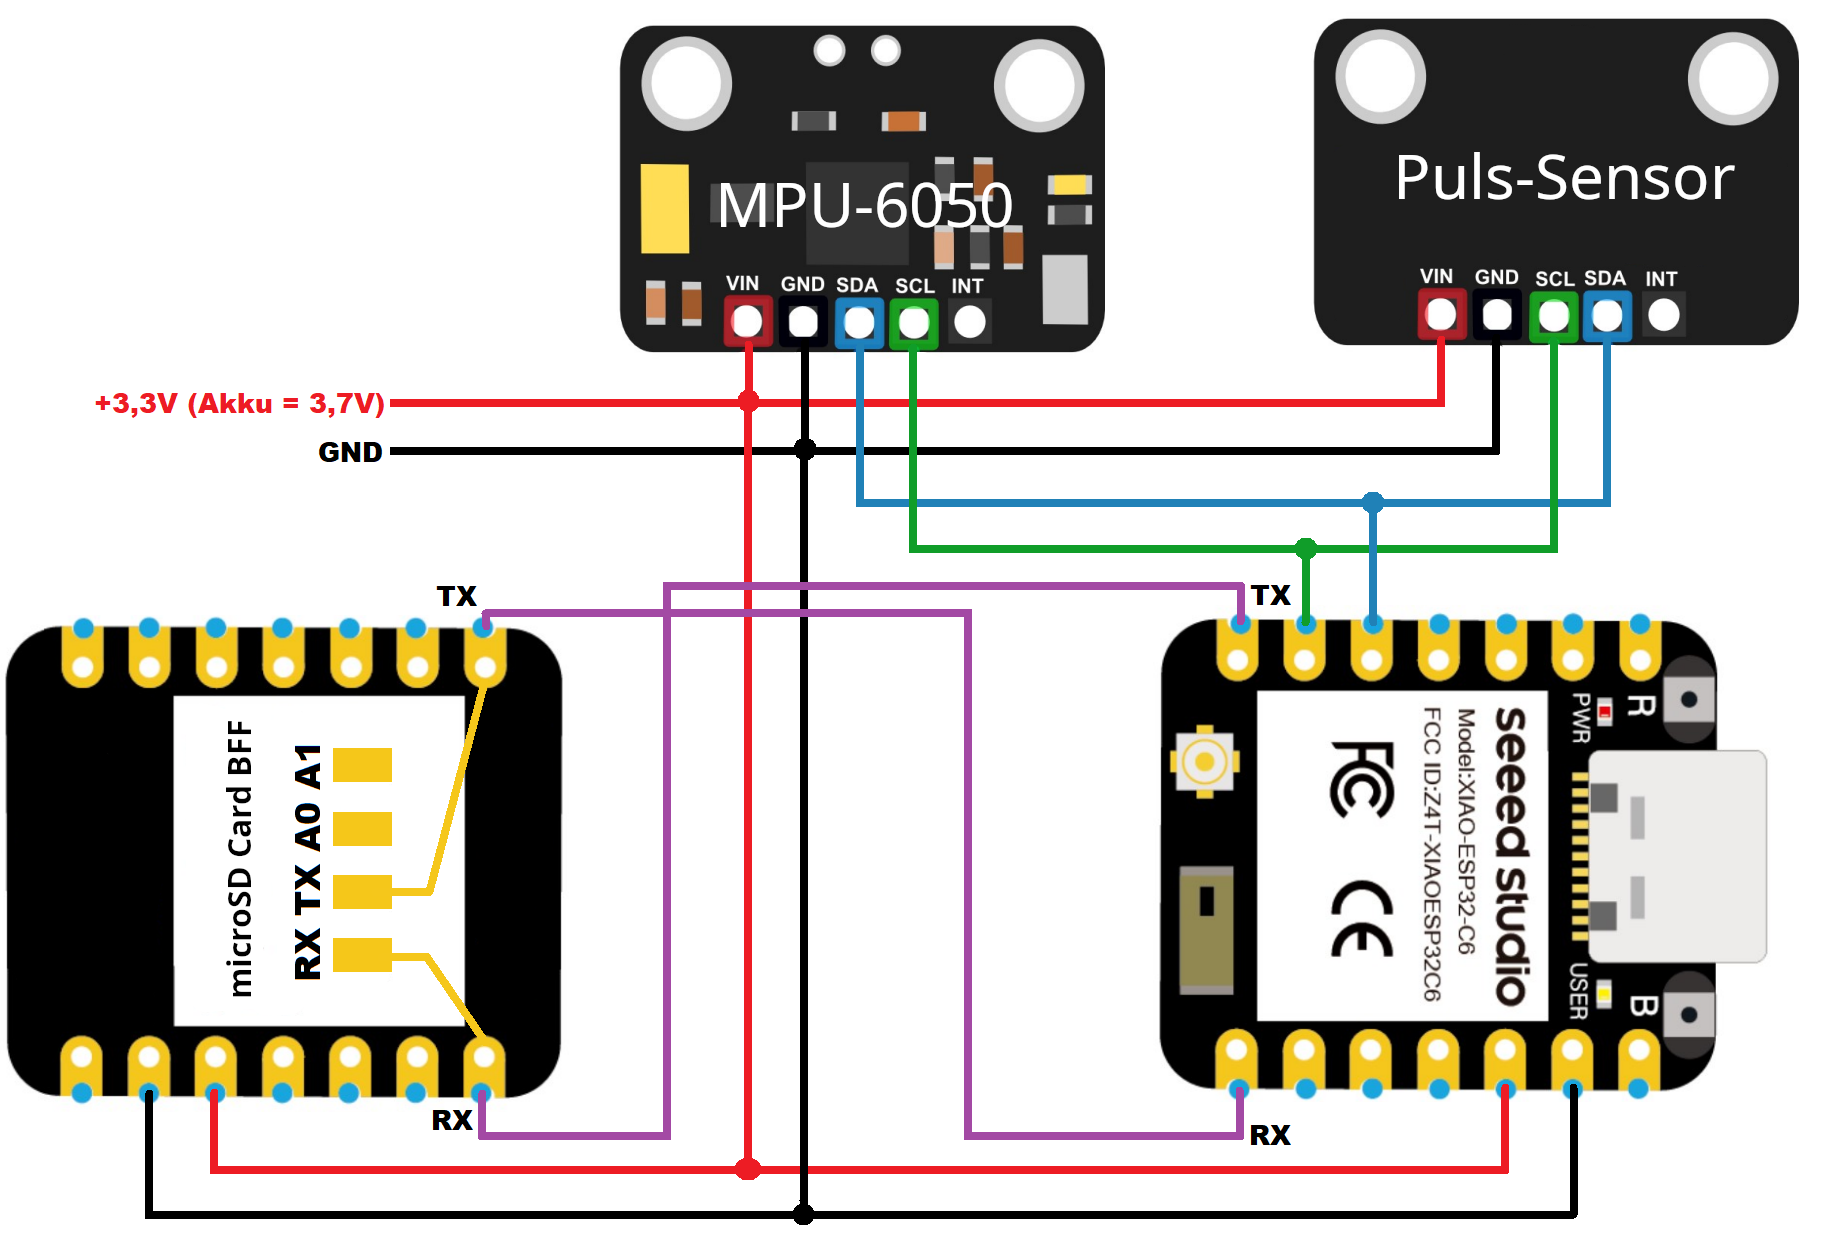
\includegraphics[width=\textwidth]{images/Schaltplan_v1.png}
        \caption{Schaltplan Smartwatch}
        \label{fig:Schaltplan Smartwatch}
    \end{subfigure}
    \begin{subfigure}{0.34\textwidth}
        \centering
        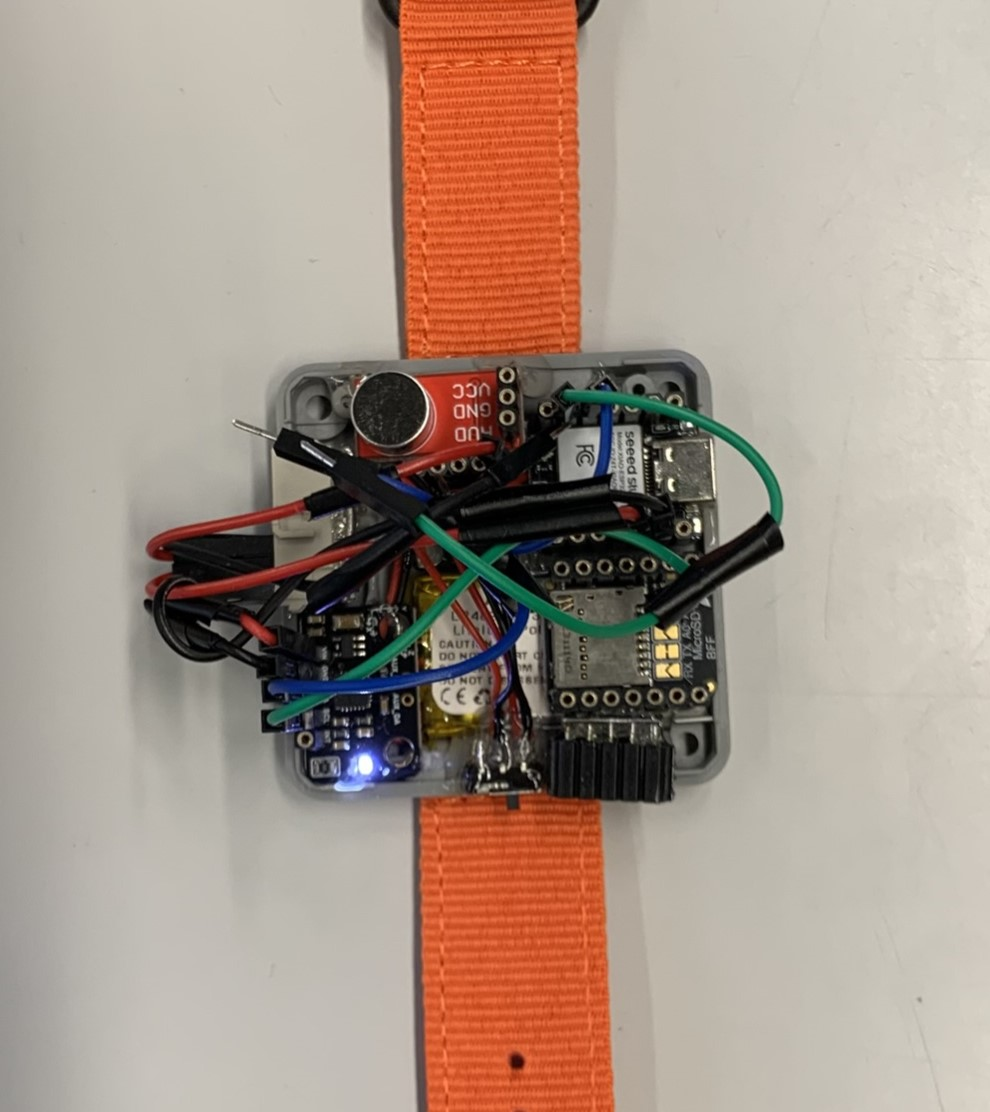
\includegraphics[width=\textwidth]{images/verkabelte_Smartwatch_cropped.JPEG}
        \caption{verkabelte Smartwatch}
        \label{fig:verkabelte Smartwatch}
    \end{subfigure}
\end{figure}
An den Mikrocontroller haben wir einen Puls-Sensor, den MPU-6050, ein 3-Achsen Gyroskop und Beschleunigungssensor, sowie einen microSD Kartenslot angeschlossen.

\noindent Zur Stromversorgung haben wir die Sensoren, den microSD Kartenslot und den Mikrocontroller mit 3,3V + Ground (im Schaltplan Rot + Schwarz) verbunden, zur Kommunikation zwischen dem Mikrokontroller und dem Puls-Sensor und dem MPU-6050 benutzen wir I2C (im Schaltplan Grün und Blau).

\noindent Die microSD Karte ist für lesende und schreibende Kommunikation mit 2 Rx Tx Verbindungen an den Mikrocontroller angeschlossen (im Schaltplan Lila).

\noindent Zur vereinfachten Verkabelung sind zwei Steckleisten auf der Uhr befestigt über die einmal die Stromversorgung und einmal die I2C Kabel gesteckt wurden.

\subsection{Stromverbrauch der Uhr:}
der Akku umfasst 700 mAh, der MPU6050 benötigt 4 mA  und der ESP32C6 im Worst Case 240mA da wir wlan für http benötigen.
Daraus ergibt sich bei unserer Verwendung für die Uhr eine Laufzeit von 2,8h.

\clearpage

\section{Datenübertragung}
Die Datenübertragung findet als HTTP GET Anfrage an den Webserver der Smartwatch statt. Die Smartwatch liefert dann einen JSON String von Datensätzen.

\noindent
Ein Datensatz enthält einen Timestamp, Acceleration x,y und z Achse, Gyroskop x,y und z Achse sowie ein Pulssensor Messwert in Folgendem Format:

\clearpage

\end{document}